% Created by tikzDevice version 0.12 on 2019-02-27 15:56:39
% !TEX encoding = UTF-8 Unicode
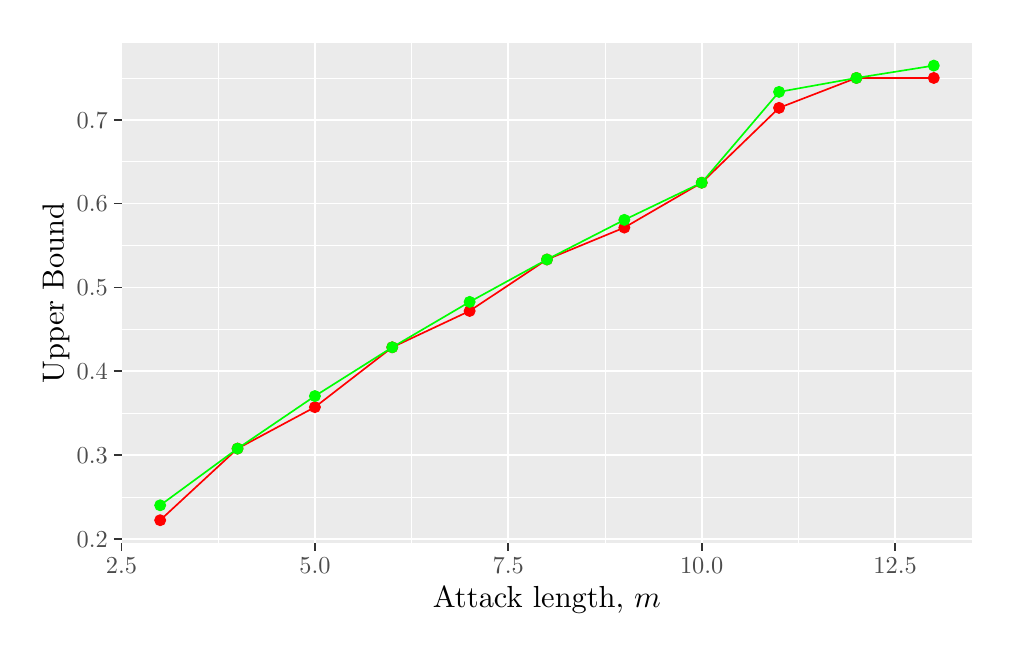
\begin{tikzpicture}[x=1pt,y=1pt]
\definecolor{fillColor}{RGB}{255,255,255}
\path[use as bounding box,fill=fillColor,fill opacity=0.00] (0,0) rectangle (346.90,216.81);
\begin{scope}
\path[clip] (  0.00,  0.00) rectangle (346.90,216.81);
\definecolor{drawColor}{RGB}{255,255,255}
\definecolor{fillColor}{RGB}{255,255,255}

\path[draw=drawColor,line width= 0.6pt,line join=round,line cap=round,fill=fillColor] (  0.00,  0.00) rectangle (346.90,216.81);
\end{scope}
\begin{scope}
\path[clip] ( 33.91, 30.62) rectangle (341.40,211.31);
\definecolor{fillColor}{gray}{0.92}

\path[fill=fillColor] ( 33.91, 30.62) rectangle (341.40,211.31);
\definecolor{drawColor}{RGB}{255,255,255}

\path[draw=drawColor,line width= 0.3pt,line join=round] ( 33.91, 47.24) --
	(341.40, 47.24);

\path[draw=drawColor,line width= 0.3pt,line join=round] ( 33.91, 77.52) --
	(341.40, 77.52);

\path[draw=drawColor,line width= 0.3pt,line join=round] ( 33.91,107.80) --
	(341.40,107.80);

\path[draw=drawColor,line width= 0.3pt,line join=round] ( 33.91,138.08) --
	(341.40,138.08);

\path[draw=drawColor,line width= 0.3pt,line join=round] ( 33.91,168.36) --
	(341.40,168.36);

\path[draw=drawColor,line width= 0.3pt,line join=round] ( 33.91,198.64) --
	(341.40,198.64);

\path[draw=drawColor,line width= 0.3pt,line join=round] ( 68.85, 30.62) --
	( 68.85,211.31);

\path[draw=drawColor,line width= 0.3pt,line join=round] (138.73, 30.62) --
	(138.73,211.31);

\path[draw=drawColor,line width= 0.3pt,line join=round] (208.62, 30.62) --
	(208.62,211.31);

\path[draw=drawColor,line width= 0.3pt,line join=round] (278.50, 30.62) --
	(278.50,211.31);

\path[draw=drawColor,line width= 0.6pt,line join=round] ( 33.91, 32.10) --
	(341.40, 32.10);

\path[draw=drawColor,line width= 0.6pt,line join=round] ( 33.91, 62.38) --
	(341.40, 62.38);

\path[draw=drawColor,line width= 0.6pt,line join=round] ( 33.91, 92.66) --
	(341.40, 92.66);

\path[draw=drawColor,line width= 0.6pt,line join=round] ( 33.91,122.94) --
	(341.40,122.94);

\path[draw=drawColor,line width= 0.6pt,line join=round] ( 33.91,153.22) --
	(341.40,153.22);

\path[draw=drawColor,line width= 0.6pt,line join=round] ( 33.91,183.50) --
	(341.40,183.50);

\path[draw=drawColor,line width= 0.6pt,line join=round] ( 33.91, 30.62) --
	( 33.91,211.31);

\path[draw=drawColor,line width= 0.6pt,line join=round] (103.79, 30.62) --
	(103.79,211.31);

\path[draw=drawColor,line width= 0.6pt,line join=round] (173.67, 30.62) --
	(173.67,211.31);

\path[draw=drawColor,line width= 0.6pt,line join=round] (243.56, 30.62) --
	(243.56,211.31);

\path[draw=drawColor,line width= 0.6pt,line join=round] (313.44, 30.62) --
	(313.44,211.31);
\definecolor{drawColor}{RGB}{255,0,0}
\definecolor{fillColor}{RGB}{255,0,0}

\path[draw=drawColor,line width= 0.4pt,line join=round,line cap=round,fill=fillColor] ( 47.88, 38.83) circle (  1.96);

\path[draw=drawColor,line width= 0.4pt,line join=round,line cap=round,fill=fillColor] ( 75.84, 64.71) circle (  1.96);

\path[draw=drawColor,line width= 0.4pt,line join=round,line cap=round,fill=fillColor] (103.79, 79.69) circle (  1.96);

\path[draw=drawColor,line width= 0.4pt,line join=round,line cap=round,fill=fillColor] (131.74,101.31) circle (  1.96);

\path[draw=drawColor,line width= 0.4pt,line join=round,line cap=round,fill=fillColor] (159.70,114.44) circle (  1.96);

\path[draw=drawColor,line width= 0.4pt,line join=round,line cap=round,fill=fillColor] (187.65,133.04) circle (  1.96);

\path[draw=drawColor,line width= 0.4pt,line join=round,line cap=round,fill=fillColor] (215.60,144.57) circle (  1.96);

\path[draw=drawColor,line width= 0.4pt,line join=round,line cap=round,fill=fillColor] (243.56,160.79) circle (  1.96);

\path[draw=drawColor,line width= 0.4pt,line join=round,line cap=round,fill=fillColor] (271.51,187.83) circle (  1.96);

\path[draw=drawColor,line width= 0.4pt,line join=round,line cap=round,fill=fillColor] (299.47,198.64) circle (  1.96);

\path[draw=drawColor,line width= 0.4pt,line join=round,line cap=round,fill=fillColor] (327.42,198.64) circle (  1.96);

\path[draw=drawColor,line width= 0.6pt,line join=round] ( 47.88, 38.83) --
	( 75.84, 64.71) --
	(103.79, 79.69) --
	(131.74,101.31) --
	(159.70,114.44) --
	(187.65,133.04) --
	(215.60,144.57) --
	(243.56,160.79) --
	(271.51,187.83) --
	(299.47,198.64) --
	(327.42,198.64);
\definecolor{drawColor}{RGB}{0,255,0}
\definecolor{fillColor}{RGB}{0,255,0}

\path[draw=drawColor,line width= 0.4pt,line join=round,line cap=round,fill=fillColor] ( 47.88, 44.22) circle (  1.96);

\path[draw=drawColor,line width= 0.4pt,line join=round,line cap=round,fill=fillColor] ( 75.84, 64.71) circle (  1.96);

\path[draw=drawColor,line width= 0.4pt,line join=round,line cap=round,fill=fillColor] (103.79, 83.69) circle (  1.96);

\path[draw=drawColor,line width= 0.4pt,line join=round,line cap=round,fill=fillColor] (131.74,101.31) circle (  1.96);

\path[draw=drawColor,line width= 0.4pt,line join=round,line cap=round,fill=fillColor] (159.70,117.72) circle (  1.96);

\path[draw=drawColor,line width= 0.4pt,line join=round,line cap=round,fill=fillColor] (187.65,133.04) circle (  1.96);

\path[draw=drawColor,line width= 0.4pt,line join=round,line cap=round,fill=fillColor] (215.60,147.36) circle (  1.96);

\path[draw=drawColor,line width= 0.4pt,line join=round,line cap=round,fill=fillColor] (243.56,160.79) circle (  1.96);

\path[draw=drawColor,line width= 0.4pt,line join=round,line cap=round,fill=fillColor] (271.51,193.60) circle (  1.96);

\path[draw=drawColor,line width= 0.4pt,line join=round,line cap=round,fill=fillColor] (299.47,198.64) circle (  1.96);

\path[draw=drawColor,line width= 0.4pt,line join=round,line cap=round,fill=fillColor] (327.42,203.10) circle (  1.96);

\path[draw=drawColor,line width= 0.6pt,line join=round] ( 47.88, 44.22) --
	( 75.84, 64.71) --
	(103.79, 83.69) --
	(131.74,101.31) --
	(159.70,117.72) --
	(187.65,133.04) --
	(215.60,147.36) --
	(243.56,160.79) --
	(271.51,193.60) --
	(299.47,198.64) --
	(327.42,203.10);
\end{scope}
\begin{scope}
\path[clip] (  0.00,  0.00) rectangle (346.90,216.81);
\definecolor{drawColor}{gray}{0.30}

\node[text=drawColor,anchor=base east,inner sep=0pt, outer sep=0pt, scale=  0.88] at ( 28.96, 29.10) {0.2};

\node[text=drawColor,anchor=base east,inner sep=0pt, outer sep=0pt, scale=  0.88] at ( 28.96, 59.38) {0.3};

\node[text=drawColor,anchor=base east,inner sep=0pt, outer sep=0pt, scale=  0.88] at ( 28.96, 89.66) {0.4};

\node[text=drawColor,anchor=base east,inner sep=0pt, outer sep=0pt, scale=  0.88] at ( 28.96,119.94) {0.5};

\node[text=drawColor,anchor=base east,inner sep=0pt, outer sep=0pt, scale=  0.88] at ( 28.96,150.22) {0.6};

\node[text=drawColor,anchor=base east,inner sep=0pt, outer sep=0pt, scale=  0.88] at ( 28.96,180.50) {0.7};
\end{scope}
\begin{scope}
\path[clip] (  0.00,  0.00) rectangle (346.90,216.81);
\definecolor{drawColor}{gray}{0.20}

\path[draw=drawColor,line width= 0.6pt,line join=round] ( 31.16, 32.10) --
	( 33.91, 32.10);

\path[draw=drawColor,line width= 0.6pt,line join=round] ( 31.16, 62.38) --
	( 33.91, 62.38);

\path[draw=drawColor,line width= 0.6pt,line join=round] ( 31.16, 92.66) --
	( 33.91, 92.66);

\path[draw=drawColor,line width= 0.6pt,line join=round] ( 31.16,122.94) --
	( 33.91,122.94);

\path[draw=drawColor,line width= 0.6pt,line join=round] ( 31.16,153.22) --
	( 33.91,153.22);

\path[draw=drawColor,line width= 0.6pt,line join=round] ( 31.16,183.50) --
	( 33.91,183.50);
\end{scope}
\begin{scope}
\path[clip] (  0.00,  0.00) rectangle (346.90,216.81);
\definecolor{drawColor}{gray}{0.20}

\path[draw=drawColor,line width= 0.6pt,line join=round] ( 33.91, 27.87) --
	( 33.91, 30.62);

\path[draw=drawColor,line width= 0.6pt,line join=round] (103.79, 27.87) --
	(103.79, 30.62);

\path[draw=drawColor,line width= 0.6pt,line join=round] (173.67, 27.87) --
	(173.67, 30.62);

\path[draw=drawColor,line width= 0.6pt,line join=round] (243.56, 27.87) --
	(243.56, 30.62);

\path[draw=drawColor,line width= 0.6pt,line join=round] (313.44, 27.87) --
	(313.44, 30.62);
\end{scope}
\begin{scope}
\path[clip] (  0.00,  0.00) rectangle (346.90,216.81);
\definecolor{drawColor}{gray}{0.30}

\node[text=drawColor,anchor=base,inner sep=0pt, outer sep=0pt, scale=  0.88] at ( 33.91, 19.66) {2.5};

\node[text=drawColor,anchor=base,inner sep=0pt, outer sep=0pt, scale=  0.88] at (103.79, 19.66) {5.0};

\node[text=drawColor,anchor=base,inner sep=0pt, outer sep=0pt, scale=  0.88] at (173.67, 19.66) {7.5};

\node[text=drawColor,anchor=base,inner sep=0pt, outer sep=0pt, scale=  0.88] at (243.56, 19.66) {10.0};

\node[text=drawColor,anchor=base,inner sep=0pt, outer sep=0pt, scale=  0.88] at (313.44, 19.66) {12.5};
\end{scope}
\begin{scope}
\path[clip] (  0.00,  0.00) rectangle (346.90,216.81);
\definecolor{drawColor}{RGB}{0,0,0}

\node[text=drawColor,anchor=base,inner sep=0pt, outer sep=0pt, scale=  1.10] at (187.65,  7.44) {Attack length, $m$};
\end{scope}
\begin{scope}
\path[clip] (  0.00,  0.00) rectangle (346.90,216.81);
\definecolor{drawColor}{RGB}{0,0,0}

\node[text=drawColor,rotate= 90.00,anchor=base,inner sep=0pt, outer sep=0pt, scale=  1.10] at ( 13.02,120.96) {Upper Bound};
\end{scope}
\end{tikzpicture}
